% Provenance (never printed): see sources/outline_sources.md (Year 2: the long-term carbon cycle
% and the silicate-weathering thermostat; Palaeozoic glaciations; the Cretaceous greenhouse; the
% PETM; Cenozoic cooling). Reservoirs from IPCC AR6 WG1 Figure 5.12; long-term fluxes after Derry
% (2024); weathering laws after Colbourn and others (2013); Phanerozoic CO2 after Foster and
% others (2017); Phanerozoic temperatures after Judd and others (2024); Cenozoic isotopes from
% CENOGRID (Westerhold 2020); the Eocene--Oligocene transition after Hutchinson and others (2021);
% the PETM after AR6 WG1 chapters 2 and 5. The thermostat model, its curves and every number of
% the exercises and problem from figdata/bachelor-2/deeptime.py and the Book 4 second-writer
% scratch calculator calc/ch26.py.
\chapter{El clima a lo largo del tiempo geológico}\label{ch:b2:deep-time-climate}

Hace cincuenta millones de años no había ningún casquete de hielo en toda la Tierra. El aire contenía más de
mil partes por millón de dióxido de carbono, los polos se habían calentado mucho más que el ecuador y
crecían bosques de tipo casi tropical a \ang{70}~S, a lo largo de los meses de la noche polar. Hace treinta y cuatro
millones de años el hielo se extendió sobre la Antártida, y nunca se ha retirado. A lo largo de los cientos de millones
de años registrados en las rocas, la Tierra ha oscilado entre mundos así, con hielo y sin él; y sin embargo
nunca ha evaporado sus océanos ni se ha congelado para siempre desde las bolas de nieve del
\cref{ch:b2:precambrian-earth}. Este capítulo sigue el carbono que fija esos climas, el ciclo lento
que lo traslada entre el aire y las rocas, y el termostato que mantiene el planeta
habitable.
% ledger: ipcc:ref-periods, ar6ch2:cenozoic, hutchinson21:eot

\begin{recall}
\textbf{De los volúmenes escolares}: el efecto invernadero y el forzamiento radiativo; el forzamiento del
dióxido de carbono crece con el logaritmo de su concentración, \qty{3.93}{W.m^{-2}} por duplicación;
la sensibilidad climática de equilibrio, con una mejor estimación de \qty{3}{\celsius}; la desgasificación; los ciclos glaciares
y el Último Máximo Glacial. \textbf{Del volumen de primer año}: la meteorización química y la
hidrólisis de los silicatos; los minerales de la arcilla; los fangos carbonatados, la lisoclina y la profundidad
de compensación de los carbonatos. \textbf{De capítulos anteriores}: el Sol joven débil y la \omterm{def:b2:precambrian-earth:snowball}{Tierra bola de nieve}
(\cref{ch:b2:precambrian-earth}); la \omterm{def:b2:phanerozoic-earth:palaeogeography}{paleogeografía} y los \omterm{def:b2:phanerozoic-earth:oae}{eventos anóxicos oceánicos}
(\cref{ch:b2:phanerozoic-earth}); los indicadores climáticos, el $\delta^{18}$O y el \omterm{def:b2:climate-proxies:ice-volume}{efecto del volumen de hielo}
(\cref{ch:b2:climate-proxies}); el forzamiento orbital (\cref{ch:b2:orbital-forcing}). El ciclo del carbono,
sus reservorios y el tiempo de residencia corresponden a los libros de biología; la ley de Arrhenius, a los
libros de química.
\end{recall}
% ledger: ipcc:erf-2xco2, ipcc:log-co2, ipcc:ecs

\section{El ciclo del carbono a largo plazo}\label{sec:b2:deep-time-climate:cycle}

\subsection*{Reservorios y flujos}

\begin{definition}[Ciclo del carbono a largo plazo; ciclo carbonato--silicato]\label{def:b2:deep-time-climate:carbon-cycle}
El \emph{ciclo del carbono a largo plazo}\index{ciclo del carbono a largo plazo} es el intercambio de carbono entre
los reservorios superficiales (atmósfera, océano, biosfera y suelos) y la Tierra sólida: la desgasificación volcánica y
metamórfica, la meteorización de las rocas y el enterramiento de carbonato y de carbono orgánico en
sedimentos que después se convierten en roca o son subducidos. Sus flujos son pequeños frente a los reservorios
superficiales y actúan a lo largo de $10^5$ a $10^8$ años. El \emph{ciclo
carbonato--silicato}\index{ciclo carbonato--silicato} es su parte inorgánica: el dióxido de carbono sale del manto
y de la corteza en los volcanes, es consumido por la meteorización de las rocas silicatadas, se deposita en el
fondo marino como carbonato y vuelve a la superficie cuando ese carbonato es metamorfizado o
subducido y desgasificado.
\end{definition}
% ledger: derry24:fluxes, derry24:subduction, colbourn13:timescale

Los libros de biología siguen el carbono a través de la fotosíntesis, la respiración y el océano a lo largo de años o
siglos. A la escala de tiempo de la historia del clima, el cuadro se amplía hasta incluir las rocas. Antes de
la era industrial la atmósfera contenía \qty{591}{PgC} (petagramos, o miles de millones de toneladas, de carbono);
el océano contenía \num{38700}, casi todo como carbono inorgánico disuelto en las aguas intermedias y
profundas (\num{37100}); la vegetación, los suelos y el permafrost contenían \num{3350} entre todos. Los
reservorios superficiales activos contienen en conjunto unos \num{3.5e6} teramoles de carbono, unos
\qty{42000}{PgC}. Las rocas sedimentarias también contienen carbono, en forma de caliza y de materia orgánica
dispersa en las lutitas, y solo lo intercambian lentamente con la superficie.
% ledger: ar6ch5:fig512, derry24:residence

Una estimación moderna de las entradas y las salidas, en teramoles de carbono al año ($\qty{1}{Tmol}$ de
carbono son \qty{0.012}{PgC}), es la siguiente. Hacia el océano y la atmósfera: la desgasificación volcánica en las
dorsales oceánicas (1.3), las \omterm{def:b2:oceanic-islands:stages}{islas oceánicas} (1.3), los arcos (4.5) y los rifts continentales (4.2), unos 11 en
total; la desgasificación metamórfica, de 2 a 4; la meteorización de carbonatos antiguos, 12.3, y la oxidación de
carbono orgánico antiguo expuesto por la erosión, 8.1, con 2.0 de metano geológico: \num{36.7} en total.
Salen de ellos: la sedimentación de carbonatos, unos 26, y el enterramiento de carbono orgánico, unos 16. Los dos
lados se equilibran dentro de sus incertidumbres. La desgasificación del interior de la Tierra aporta poco más de un
tercio de la entrada (\cref{exo:b2:deep-time-climate:2}); el resto es carbono sedimentario antiguo que
vuelve a dar la vuelta. Otras estimaciones del flujo volcánico son más bajas: \qty{0.1}{PgC} al año
(unos 8 Tmol) en el balance global de carbono del IPCC, o \qty{0.26}{Gt} de dióxido de carbono (unos 6
Tmol de carbono) en una revisión del Servicio Geológico de Estados Unidos: la entrada volcánica se conoce con un
margen de un factor dos.
% ledger: derry24:fluxes, ar6ch5:fig512, usgs:volcanic-co2

\begin{omfigure}
\centering
\begin{tikzpicture}[font=\scriptsize, >={Stealth[length=2mm]},
  box/.style={draw, thick, rounded corners=2pt, align=center, inner sep=4pt},
  up/.style={->, very thick, omThm}, down/.style={<-, very thick, omDef},
  lab/.style={midway, above, sloped, font=\scriptsize}]
% reservoirs: ar6ch5:fig512; active reservoirs derry24:residence; fluxes derry24:fluxes, derry24:subduction
\draw[thick, rounded corners=2pt, fill=blue!6] (-6.3,0) rectangle (6.0,2.6);
\node[anchor=north west, font=\small\bfseries] at (-6.2,2.55) {reservorios superficiales, unos \qty{42000}{PgC}};
\node[box, fill=white] (atm) at (-4.6,1.45) {atmósfera\\\qty{591}{PgC}};
\node[box, fill=white] (oc) at (0.6,1.45) {océano\\\qty{38700}{PgC}};
\node[box, fill=white] (land) at (4.3,1.45) {vegetación, suelos,\\permafrost \qty{3350}{PgC}};
\draw[->, very thick, omProp] (atm.east) -- (oc.west);
\node[align=center, text=omProp] at (-2.0,0.6) {meteorización de silicatos 11--12, como bicarbonato};
\draw[<->, thick, black!50] (oc.east) -- (land.west);
% sedimentary rocks and mantle
\node[box, fill=brown!12, minimum width=5.7cm, minimum height=1.1cm] (rock) at (-3.35,-4.55) {rocas sedimentarias:\\carbonato y carbono orgánico};
\node[box, fill=orange!15, minimum width=3.0cm, minimum height=1.1cm] (mantle) at (4.3,-4.55) {manto};
% inputs (red, up) and outputs (blue, drawn upwards with the tip at the start)
\draw[up] (-5.7,-4.0) -- node[lab] {\shortstack{meteorización de\\carbonatos 12.3}} (-5.7,0);
\draw[up] (-4.8,-4.0) -- node[lab] {\shortstack{C orgánico antiguo\\oxidado 8.1}} (-4.8,0);
\draw[up] (-3.9,-4.0) -- node[lab] {metano geológico 2.0} (-3.9,0);
\draw[up] (-3.0,-4.0) -- node[lab] {\shortstack{desgasificación\\metamórfica 2--4}} (-3.0,0);
\draw[down] (-1.9,-4.0) -- node[lab] {\shortstack{sedimentación de\\carbonatos 26}} (-1.9,0);
\draw[down] (-1.0,-4.0) -- node[lab] {\shortstack{enterramiento de\\C orgánico 16}} (-1.0,0);
\draw[up] (4.3,-4.0) -- node[lab] {volcanes, rifts 11.3} (4.3,0);
\draw[->, very thick, black!70] (rock.east) -- node[above] {subducción 4--6} (mantle.west);
\end{tikzpicture}
\par\smallskip{\small El \omterm{def:b2:deep-time-climate:carbon-cycle}{ciclo del carbono a largo plazo}, con los reservorios preindustriales del balance global
de carbono del IPCC y los flujos actuales de una síntesis de 2024, en teramoles de carbono al año
(\qty{1}{Tmol.yr^{-1}} = \qty{0.012}{PgC.yr^{-1}}). Rojo: entradas a los reservorios superficiales; azul:
salidas. La meteorización de silicatos no sale de la superficie: traslada carbono del aire al
océano como bicarbonato, que después sale como sedimento carbonatado.}
\end{omfigure}

Divididos por el flujo que los atraviesa, los \qty{3.5e6}{Tmol} de los reservorios superficiales dan un
tiempo de residencia del carbono de 8 a \num{9e4} años. El carbono que entra en el océano y el aire vuelve a enterrarse
en unos cien mil años, un parpadeo a la escala de este capítulo: los reservorios superficiales
siguen de cerca las lentas entradas y salidas, y cualquier desequilibrio duradero entre ellas
cambia el dióxido de carbono del aire.
% ledger: derry24:residence

\subsection*{La meteorización de carbonatos y de silicatos}

La lluvia disuelve dióxido de carbono y ataca las rocas, como se describió en el volumen de primer año. Dos tipos de roca
se comportan de forma muy distinta. La meteorización de una caliza lleva al agua un dióxido de carbono del aire y un
carbono de la roca; cuando un organismo marino construye su concha con los productos,
un carbono vuelve al aire:
\[
  \ce{CaCO3 + CO2 + H2O -> Ca^{2+} + 2 HCO3^-} , \qquad
  \ce{Ca^{2+} + 2 HCO3^- -> CaCO3 + CO2 + H2O} .
\]
El viaje de ida y vuelta es nulo para el aire. La meteorización de un silicato, escrita aquí con la wollastonita como
representante de los silicatos cálcicos del granito y del basalto, también consume dióxido de carbono, pero no aporta
ninguno desde la roca:
\[
  \ce{CaSiO3 + 2 CO2 + H2O -> Ca^{2+} + 2 HCO3^- + SiO2} ,
\]
y el carbonato formado a partir de ella devuelve solo una de las dos moléculas:
\[
  \ce{CaSiO3 + CO2 -> CaCO3 + SiO2} \quad\text{(neta)} .
\]
Cada mol de silicato de calcio o de magnesio meteorizado en tierra firme fija así un mol de dióxido de carbono
en roca carbonatada. Por eso la sedimentación de carbonatos, unos 26, supera a la meteorización de carbonatos,
12.3, aproximadamente en los 11 a 12 teramoles al año que consume la meteorización de silicatos; y es la
meteorización de silicatos, no la de carbonatos, la que equilibra a los volcanes a lo largo de millones de años.
% ledger: colbourn13:timescale, derry24:fluxes

\section{El termostato de la meteorización de los silicatos}\label{sec:b2:deep-time-climate:thermostat}

\subsection*{Una retroalimentación negativa}

La meteorización de silicatos es una reacción química y, como la mayoría, es más rápida cuando hace calor. El calor
trae además más lluvia y más escorrentía, que se llevan los productos y aportan agua nueva a la
roca. La velocidad aumenta, por tanto, con la temperatura; y la temperatura aumenta con el dióxido de carbono del
aire. Un planeta que gana dióxido de carbono se calienta, se meteoriza más deprisa y lo vuelve a perder.

\begin{definition}[Termostato de la meteorización de los silicatos]\label{def:b2:deep-time-climate:thermostat}
El \emph{termostato de la meteorización de los silicatos}\index{termostato de la meteorizacion de los silicatos@termostato de la meteorización de los silicatos} es la retroalimentación
negativa entre el clima y el \omterm{def:b2:deep-time-climate:carbon-cycle}{ciclo del carbono a largo plazo}: la meteorización de las rocas silicatadas, que
retira dióxido de carbono de la atmósfera hacia la roca carbonatada, aumenta con la temperatura y la
escorrentía, de modo que una subida del dióxido de carbono atmosférico aumenta la velocidad de su propia retirada y una
bajada la reduce. A lo largo de $10^5$ a $10^6$ años, devuelve la retirada al equilibrio con la
desgasificación.
\end{definition}
% ledger: colbourn13:timescale, colbourn13:weathering, hutchinson21:gateways

La dependencia de la temperatura es la de la ley de Arrhenius de los libros de química. Con una energía de
activación $E_{\text a}$ para la disolución de los silicatos de calcio y de magnesio, el flujo de meteorización a
una temperatura $T$ cercana a una referencia $T_0$ es
\[
  W = W_0 \exp\Bigl[-\frac{E_{\text a}}{R}\Bigl(\frac1T - \frac1{T_0}\Bigr)\Bigr]
  \approx W_0\, e^{k_T (T - T_0)}, \qquad k_T = \frac{E_{\text a}}{R T_0^2},
\]
ya que $1/T - 1/T_0 \approx -(T - T_0)/T_0^2$. La disolución en laboratorio da $E_{\text a} =
\qty{63}{kJ.mol^{-1}}$, y con $T_0 = \qty{288}{K}$, $k_T = \qty{0.09}{K^{-1}}$: el flujo crece
alrededor de un \qty{9}{\percent} por cada grado; a menos de diez grados de $T_0$, la aproximación se aparta
de la ley exacta menos de un \qty{3}{\percent} (\cref{exo:b2:deep-time-climate:6}). Una estimación de campo es
$74 \pm \qty{29}{kJ.mol^{-1}}$, así que la sensibilidad es incierta en un factor dos aproximadamente. La escorrentía
se suma a ella: con un flujo proporcional a $(R/R_0)^{0.65}$ y una escorrentía que aumenta un
\qty{4.5}{\percent} por grado, la sensibilidad combinada pasa a ser $k = 0.09 + 0.65\times0.045 =
\qty{0.119}{K^{-1}}$.
% ledger: colbourn13:weathering
% values: k_run 0.11925 (deeptime.py)

\subsection*{Un modelo de una caja}

Para ver con qué rapidez actúa el termostato, sígase el exceso de carbono $M$ que el océano y la atmósfera
contienen por encima de un estado estacionario. A los pocos miles de años de una perturbación, el océano y los carbonatos
del fondo marino han retirado del aire la mayor parte de un exceso; para una emisión de \qty{4000}{PgC}, alrededor de un
\qty{8}{\percent} permanece en el aire hasta que la meteorización de silicatos lo retira. Llámese $f$ a esa
fracción y $A_0 = \qty{591}{PgC}$ al carbono preindustrial del aire, de modo que el dióxido de carbono
del aire es $C = C_0(1 + fM/A_0)$. El calentamiento sigue la ley logarítmica con la sensibilidad climática
$S$, $\Delta T = S\log_2(C/C_0)$, y la meteorización sigue la ley exponencial anterior.
% ledger: colbourn13:timescale, ar6ch5:fig512, ipcc:ecs, ipcc:log-co2

\begin{proposition}[Estado estacionario y constante de tiempo del termostato]\label{prop:b2:deep-time-climate:thermostat}
Sea el exceso de carbono $M$ del sistema océano--atmósfera, que evoluciona según
\[
  \frac{\mathrm dM}{\mathrm dt} = V - W_0\,e^{k\,\Delta T(M)}, \qquad
  \Delta T(M) = S\log_2\Bigl(1 + \frac{fM}{A_0}\Bigr),
\]
donde $V$ es la desgasificación y $W_0$ la meteorización para $M = 0$.
\begin{enumerate}
  \item El estado estacionario cumple $\Delta T^* = \ln(V/W_0)/k$, sean cuales sean $S$ y $f$.
  \item Si $V = W_0$, un exceso pequeño decrece como $M(t) = M(0)\,e^{-t/\tau}$ con
        \[
          \tau = \frac{A_0 \ln 2}{f\,k\,S\,W_0} .
        \]
\end{enumerate}
\end{proposition}

\begin{proof}
(1) En un estado estacionario $\mathrm dM/\mathrm dt = 0$, así que $W_0e^{k\Delta T^*} = V$ y $\Delta T^* =
\ln(V/W_0)/k$; no intervienen ni $S$ ni $f$. (2) Cerca de $M = 0$, $\log_2(1 + x) \approx x/\ln 2$, así que
$\Delta T \approx SfM/(A_0\ln 2)$ y $e^{k\Delta T} \approx 1 + kSfM/(A_0\ln2)$. Con $V = W_0$, la
ecuación se convierte en $\mathrm dM/\mathrm dt = -W_0kSfM/(A_0\ln 2) = -M/\tau$, cuya solución es la
exponencial.
\end{proof}

El primer resultado es el corazón del termostato. Fija una temperatura, no una concentración: si
los volcanes desgasifican un \qty{20}{\percent} más, la Tierra se estabiliza $\ln 1.2/0.09 = \qty{2.0}{\celsius}$
más caliente, sea cual sea su sensibilidad climática, y el dióxido de carbono se ajusta al valor que produce ese
calentamiento, aquí un \qty{60}{\percent} más. Una respuesta débil de la meteorización, una $k$ pequeña, hace un mal
termostato; una fuerte mantiene la temperatura casi fija.
% values: dT_step 2.026, C_step_ratio 1.597 (deeptime.py)

\begin{example}[La constante de tiempo del termostato]\label{ex:b2:deep-time-climate:tau}
La meteorización de silicatos consume de 11 a \qty{12}{Tmol} de carbono al año; tómese $W_0 = 11.5\times0.012011
= \qty{0.138}{PgC.yr^{-1}}$. Con $A_0 = \qty{591}{PgC}$, $f = 0.08$, $k = \qty{0.09}{K^{-1}}$ y
$S = \qty{3}{K}$,
\[
  \tau = \frac{591\times0.693}{0.08\times0.09\times3\times0.138} = \qty{1.37e5}{yr} ,
\]
unos 140 mil años. Con el factor de escorrentía, $k = 0.119$, se acorta hasta
\qty{104}{kyr}.
\end{example}
% ledger: derry24:fluxes, ar6ch5:fig512, colbourn13:timescale, colbourn13:weathering, ipcc:ecs
% values: tau_kT_kyr 137.3, tau_run_kyr 103.6 (deeptime.py)

El modelo es tosco: la fracción $f$ no es una constante, la química del océano se reduce a un solo
número y la meteorización a una sola ley global. Los modelos con un océano y unos sedimentos explícitos dan
tiempos característicos de unos \qty{200}{kyr} a un millón de años. El termostato es, por tanto, un
regulador del muy largo plazo: no actúa sobre el clima de los próximos miles de años, y
mantiene la temperatura de la Tierra dentro de unos límites a lo largo de cientos de millones.
% ledger: colbourn13:timescale

\begin{omfigure}
\centering
\begin{tikzpicture}
\begin{groupplot}[group style={group size=2 by 1, horizontal sep=1.6cm},
  omrecord, width=0.47\linewidth, height=5.4cm, xmin=0, xmax=1000,
  xlabel={tiempo (\unit{kyr})}, xtick pos=bottom, ytick pos=left,
  tick label style={font=\scriptsize}, label style={font=\small},
  legend style={draw=none, fill=white, font=\scriptsize}]
\nextgroupplot[ymin=0, ymax=5200, ylabel={exceso de carbono (\unit{PgC})},
  y tick label style={/pgf/number format/1000 sep={\,}},
  legend style={at={(0.97,0.97)}, anchor=north east}]
% computed in figdata/bachelor-2/deeptime.py part pulse; ledger: colbourn13:timescale, colbourn13:weathering, derry24:fluxes, ar6ch5:fig512, ipcc:ecs
\addplot[omThm, line width=1.2pt] table[x=t_kyr, y=M_nl] {figdata/out/bachelor-2-deeptime-pulse.dat};
\addlegendentry{modelo}
\addplot[black, densely dashed, line width=1.0pt] table[x=t_kyr, y=M_lin] {figdata/out/bachelor-2-deeptime-pulse.dat};
\addlegendentry{linealizado}
\draw[densely dotted] (axis cs:137.3,0) -- (axis cs:137.3,1839);
\node[anchor=west, font=\scriptsize] at (axis cs:145,1400) {$\tau$};
\nextgroupplot[ymin=0, ymax=2.4, ylabel={calentamiento (\unit{\celsius})},
  legend style={at={(0.97,0.03)}, anchor=south east}]
% computed in figdata/bachelor-2/deeptime.py part step
\addplot[omThm, line width=1.2pt] table[x=t_kyr, y=dT_nl] {figdata/out/bachelor-2-deeptime-step.dat};
\addlegendentry{modelo}
\addplot[black, densely dashed, line width=1.0pt] table[x=t_kyr, y=dT_lin] {figdata/out/bachelor-2-deeptime-step.dat};
\addlegendentry{linealizado}
\draw[densely dotted] (axis cs:0,2.026) -- (axis cs:1000,2.026);
\node[anchor=south east, font=\scriptsize] at (axis cs:1000,2.03) {$\ln 1.2/k$};
\end{groupplot}
\end{tikzpicture}
\par\smallskip{\small El termostato de una caja con $k = \qty{0.09}{K^{-1}}$ y $S = \qty{3}{K}$.
Izquierda: una emisión de \qty{5000}{PgC} en el instante cero, contada después de que el océano y los carbonatos hayan
retirado su parte; decrece con el tiempo característico $\tau$, al principio algo más despacio que la
ley linealizada. Derecha: la desgasificación aumentada un \qty{20}{\percent} en el instante cero; la Tierra
se calienta hacia los \qty{2.0}{\celsius} estacionarios de la \cref{prop:b2:deep-time-climate:thermostat}.}
\end{omfigure}
% values: t90_lin_kyr 316.2, t90_nl_kyr 339.9, tau_step_kyr 182.7 (deeptime.py)

El termostato explica también el Sol joven débil del \cref{ch:b2:precambrian-earth}. El Sol aumenta su brillo
en un pequeño porcentaje cada pocos cientos de millones de años, y una Tierra con un aire fijo se calentaría con él;
pero más calor significa una meteorización más rápida, que hace bajar el dióxido de carbono hasta que la temperatura
vuelve cerca del valor que fija la desgasificación. Las rocas de los últimos 420 millones de años muestran exactamente
esto, como se lee en la sección siguiente.

\section{Mundos de invernadero y mundos glaciares}\label{sec:b2:deep-time-climate:states}

\begin{definition}[Estados climáticos de invernadero y glaciar]\label{def:b2:deep-time-climate:states}
Un \emph{estado climático de invernadero}\index{estado climatico de invernadero@estado climático de invernadero} es un largo intervalo, de millones a
decenas de millones de años, sin grandes casquetes de hielo continentales, con mucho dióxido de carbono
atmosférico y una pequeña diferencia de temperatura entre el ecuador y los polos. Un \emph{estado climático
glaciar}\index{estado climatico glaciar@estado climático glaciar} es un largo intervalo con casquetes de hielo continentales en uno
o en ambos polos, menos dióxido de carbono y un fuerte gradiente entre el ecuador y los polos. La Tierra está en un
estado glaciar desde hace unos \qty{34}{Ma}.
\end{definition}
% ledger: judd24:phanda, hutchinson21:eot

\subsection*{El dióxido de carbono a lo largo de 420 millones de años}

El dióxido de carbono anterior a los testigos de hielo se lee en indicadores: los isótopos del boro y las moléculas orgánicas
del plancton marino, los estomas de las hojas fósiles, los nódulos carbonatados de los suelos antiguos. Una
compilación de 2017 de estos datos hasta \qty{420}{Ma}, suavizada, se muestra abajo con las glaciaciones. Su
tendencia a largo plazo es un descenso de unos \qty{3.4}{ppm} por millón de años, y aparecen valores cercanos al
nivel preindustrial dos veces antes de nuestra época: en el Carbonífero y el Pérmico, y
brevemente en el Cretácico superior.
% ledger: foster17:co2, data:b4-foster2017, ar6ch2:deep-co2

\begin{omfigure}
\centering
\begin{tikzpicture}
\begin{axis}[omrecord, omage, width=0.92\linewidth, height=6.4cm, xmin=0, xmax=450, ymode=log,
  ymin=80, ymax=8000, xlabel={edad (\unit{Ma})}, ylabel={dióxido de carbono (\unit{ppm})},
  xtick={0,50,...,400}, ytick={100,200,500,1000,2000,5000}, yticklabels={100,200,500,1000,2000,5000},
  xtick pos=bottom, ytick pos=left, clip=false,
  tick label style={font=\scriptsize}, label style={font=\small}]
% computed in figdata/bachelor-2/deeptime.py part co2; ledger: data:b4-foster2017, foster17:co2, judd24:phanda, hutchinson21:eot, ar6ch5:cenozoic-co2, ics:base.Ordovician, ics:base.Silurian, ics:base.Devonian, ics:base.Carboniferous, ics:base.Permian, ics:base.Triassic, ics:base.Jurassic, ics:base.Cretaceous, ics:base.Paleogene, ics:base.Neogene, ics:colour.Ordovician, ics:colour.Silurian, ics:colour.Devonian, ics:colour.Carboniferous, ics:colour.Permian, ics:colour.Triassic, ics:colour.Jurassic, ics:colour.Cretaceous, ics:colour.Paleogene, ics:colour.Neogene
\fill[blue!12] (axis cs:445.21,80) rectangle (axis cs:443.07,8000);
\fill[blue!12] (axis cs:371.1,80) rectangle (axis cs:298.89,8000);
\fill[blue!12] (axis cs:34,80) rectangle (axis cs:0,8000);
\addplot[name path=hi, draw=none, forget plot] table[x=age, y=hi68] {figdata/out/bachelor-2-deeptime-co2.dat};
\addplot[name path=lo, draw=none, forget plot] table[x=age, y=lo68] {figdata/out/bachelor-2-deeptime-co2.dat};
\addplot[omDef!25, forget plot] fill between[of=hi and lo];
\addplot[omDef, line width=1.2pt] table[x=age, y=co2] {figdata/out/bachelor-2-deeptime-co2.dat};
\addplot[black!60, densely dashed] coordinates {(0,278) (450,278)};
\node[anchor=south west, font=\scriptsize, text=black!70] at (axis cs:440,280) {preindustrial};
\node[anchor=north west, font=\scriptsize, text=blue!60!black, align=left] at (axis cs:442,7600) {Ordovícico\\superior};
\node[anchor=north, font=\scriptsize, text=blue!60!black, align=center] at (axis cs:335,7600) {glaciación del\\Paleozoico superior};
\node[anchor=north, font=\scriptsize, text=blue!60!black, align=center] at (axis cs:17,7600) {hielo\\cenozoico};
\foreach \a/\b/\c in {450/443.1/icsOrdovician, 443.1/419.62/icsSilurian, 419.62/358.86/icsDevonian, 358.86/298.9/icsCarboniferous,
  298.9/251.902/icsPermian, 251.902/201.4/icsTriassic, 201.4/143.1/icsJurassic,
  143.1/66/icsCretaceous, 66/23.04/icsPaleogene, 23.04/0/icsNeogene} {
  \edef\tmp{\noexpand\fill[\c] (axis cs:\a,80) rectangle (axis cs:\b,95);}\tmp}
\node[font=\tiny] at (axis cs:431.4,87) {S};
\node[font=\tiny] at (axis cs:389.2,87) {D};
\node[font=\tiny] at (axis cs:328.9,87) {C};
\node[font=\tiny] at (axis cs:275.4,87) {P};
\node[font=\tiny] at (axis cs:226.7,87) {T};
\node[font=\tiny] at (axis cs:172.3,87) {J};
\node[font=\tiny] at (axis cs:104.6,87) {K};
\node[font=\tiny] at (axis cs:44.5,87) {Pg};
\end{axis}
\end{tikzpicture}
\par\smallskip{\small El dióxido de carbono atmosférico a lo largo de los últimos 420 millones de años: el ajuste suavizado
(línea) a una compilación de estimaciones indirectas, con su banda del \qty{68}{\percent}, en escala
logarítmica. Bandas azules: la glaciación hirnantiense del Ordovícico superior; la glaciación del Paleozoico superior,
desde sus primeros depósitos glaciares en el Devónico final hasta su máxima extensión de hielo a finales del
Carbonífero; el hielo cenozoico desde \qty{34}{Ma}. La barra inferior muestra los periodos.}
\end{omfigure}

A lo largo de esos mismos 420 millones de años, el Sol aumentó su brillo en alrededor de un \qty{4}{\percent}, unos
\qty{50}{W.m^{-2}} a la distancia de la Tierra y \qty{9}{W.m^{-2}} de forzamiento una vez repartido sobre la
esfera y corregido por el albedo. La caída del dióxido de carbono desde unos \qty{1400}{ppm} hasta el
valor preindustrial lo compensa casi exactamente (\cref{exo:b2:deep-time-climate:7}): en términos de
forzamiento, la Tierra se ha mantenido a pocos vatios por metro cuadrado del actual durante 420 millones de años,
y sus estados glaciares llegaron cuando el forzamiento combinado del dióxido de carbono y del Sol cayó por debajo de 1
a \qty{2}{W.m^{-2}} aproximadamente. Los autores de la compilación atribuyen la compensación a la retroalimentación de la
meteorización de silicatos y a la expansión de las plantas terrestres, cuyas raíces y suelos aceleran la meteorización.
% ledger: foster17:co2, data:b4-foster2017, ipcc:erf-2xco2

\subsection*{Las glaciaciones paleozoicas}

Una reconstrucción de la temperatura media global en superficie publicada en 2024, que combina datos indirectos
con modelos climáticos, sitúa el intervalo del Fanerozoico entre \qty{11}{\celsius}, en los tiempos glaciares del
Pleistoceno superior, hace de 129 a 11.7 mil años, y \qty{36}{\celsius}, en el Turoniense, hace de 94 a \qty{89}{Ma}.
Sus intervalos cálidos y fríos siguen las glaciaciones registradas por tillitas y pavimentos estriados.
% ledger: judd24:phanda

La glaciación del Ordovícico superior, en el piso Hirnantiense (de 445.2 a \qty{443.1}{Ma}), extendió casquetes de hielo
sobre Gondwana, gran parte del cual se hallaba cerca del Polo Sur (\cref{ch:b2:phanerozoic-earth}), y
coincidió con una de las cinco grandes extinciones. Su temperatura media global, de unos
\qty{21}{\celsius} en la reconstrucción, es más cálida que la de las glaciaciones posteriores: el inmenso
\omterm{def:b2:wilson-cycle:supercontinent}{supercontinente} enfrió su interior lo suficiente para albergar casquetes de hielo de todos modos. La glaciación del Paleozoico superior es
la más larga del Fanerozoico: sus primeros depósitos glaciares son del Devónico final, sus temperaturas globales más
frías se dan en el Serpujoviense, hace unos 330 a \qty{323}{Ma}, y su máxima extensión
de hielo hacia el final del Carbonífero, de 307 a \qty{299}{Ma}. Coincide con el bajo dióxido
de carbono del Carbonífero y el Pérmico, que los autores de la compilación relacionan con un flujo volcánico más débil
o una meteorización más intensa mientras Pangea se ensamblaba y sus montañas eran altas.
% ledger: judd24:phanda, ar6ch2:deep-co2, foster17:co2, ics:base.Silurian

\subsection*{El invernadero cretácico}

El periodo más cálido de la reconstrucción es el Cretácico medio, la época de los mares altos y de los
\omterm{def:b2:phanerozoic-earth:oae}{eventos anóxicos oceánicos} del \cref{ch:b2:phanerozoic-earth}. Las estimaciones de dióxido de carbono para
esa época son desconcertantes: la compilación anterior da entre unos 450 y \qty{860}{ppm} entre 100 y
\qty{90}{Ma}, y la reconstrucción de 2024 halla una mediana de unos \qty{775}{ppm} para sus intervalos
más cálidos, menos de lo que sugieren sus temperaturas. Si el dióxido de carbono y la temperatura se separaron de verdad
entonces, o si los indicadores leen mal el aire del Cretácico, es una cuestión abierta; los autores lo llaman el «enigma
del Mesozoico».
% ledger: judd24:phanda, data:b4-foster2017

\section{El Cenozoico: del invernadero extremo al estado glaciar}\label{sec:b2:deep-time-climate:cenozoic}

El mejor registro de los últimos 66 millones de años está en los caparazones de los foraminíferos bentónicos, extraídos en testigos
del fondo del mar profundo. Su $\delta^{18}$O aumenta cuando el agua profunda se enfría y cuando los casquetes de hielo almacenan
el isótopo ligero en tierra (\cref{ch:b2:climate-proxies}). La figura siguiente muestra el registro de
referencia construido en 2020 a partir de sondeos de mar profundo, promediado sobre \qty{100}{kyr}.
% ledger: data:b4-cenogrid, ar6ch2:cenozoic

\begin{omfigure}
\centering
\begin{tikzpicture}
\begin{axis}[omrecord, omage, width=0.92\linewidth, height=6.4cm, xmin=0, xmax=67,
  ymin=-1.2, ymax=5.6, y dir=reverse, xlabel={edad (\unit{Ma})},
  ylabel={$\delta^{18}$O bentónico (\unit{\permil})}, xtick={0,10,...,60},
  xtick pos=bottom, ytick pos=left, clip=false,
  tick label style={font=\scriptsize}, label style={font=\small}]
% computed in figdata/bachelor-2/deeptime.py part ceno; ledger: data:b4-cenogrid, ar6ch2:cenozoic, ar6ch5:cenozoic-co2, hutchinson21:eot, ipcc:ref-periods, ar6ch5:petm
\fill[omThm!15] (axis cs:53,-1.2) rectangle (axis cs:49,5.6);
\fill[omThm!15] (axis cs:16.9,-1.2) rectangle (axis cs:14.7,5.6);
\addplot[black!45, line width=0.4pt] table[x=age, y=d18O] {figdata/out/bachelor-2-deeptime-ceno.dat};
\addplot[omDef, line width=1.3pt] table[x=age, y=d18O_lt] {figdata/out/bachelor-2-deeptime-ceno.dat};
\draw[omThm, thick, ->] (axis cs:55.85,-0.7) -- (axis cs:55.85,-1.15);
\node[anchor=south, font=\scriptsize, text=omThm] at (axis cs:55.85,-1.15) {PETM};
\node[anchor=north, font=\scriptsize, text=omThm] at (axis cs:51,4.6) {EECO};
\node[anchor=north, font=\scriptsize, text=omThm] at (axis cs:15.8,0.6) {MCO};
\draw[blue!60!black, densely dashed] (axis cs:33.9,-1.2) -- (axis cs:33.9,5.6);
\node[anchor=south west, font=\scriptsize, text=blue!60!black, align=left] at (axis cs:33.6,4.4)
  {hielo antártico\\desde \qty{34}{Ma}};
\draw[blue!60!black, densely dashed] (axis cs:2.7,-1.2) -- (axis cs:2.7,5.6);
\node[anchor=north west, font=\scriptsize, text=blue!60!black, align=left] at (axis cs:2.5,-0.9)
  {casquetes\\boreales};
\node[anchor=south west, font=\scriptsize, align=left] at (axis cs:66.3,5.45) {más frío,\\más hielo $\downarrow$};
\end{axis}
\end{tikzpicture}
\par\smallskip{\small $\delta^{18}$O de los foraminíferos bentónicos del mar profundo a lo largo del Cenozoico, según el
empalme de referencia CENOGRID: medias de \qty{100}{kyr} (gris) y el suavizado a largo plazo del conjunto de datos
(azul). El eje está invertido, de modo que lo más frío y con más hielo queda abajo. Sombreados: el Óptimo Climático del Eoceno
Temprano (EECO) y el Óptimo Climático del Mioceno (MCO); discontinuas: el inicio del casquete de hielo
antártico y los grandes avances de los casquetes de hielo del norte.}
\end{omfigure}

Leído de derecha a izquierda, el registro cuenta cuatro capítulos. El Cenozoico temprano se calentó, a través del
\omterm{def:b2:deep-time-climate:petm}{Máximo Térmico del Paleoceno--Eoceno}, hasta el Óptimo Climático del Eoceno Temprano, de 53 a \qty{49}{Ma}, cuando
la temperatura global estaba de 10 a \qty{18}{\celsius} por encima de la de 1850--1900 (\emph{confianza
media}, en el lenguaje del IPCC) y el dióxido de carbono entre 1150 y \qty{2500}{ppm}.
Siguió un largo enfriamiento, marcado en la transición Eoceno--Oligoceno, hace unos \qty{34}{Ma}, por un
salto de alrededor de \qty{1.5}{\permil} en el $\delta^{18}$O: el primer gran casquete de hielo sobre la Antártida, con un
enfriamiento del océano profundo del orden de \qty{2}{\celsius}. El Óptimo Climático del Mioceno, de 16.9 a
\qty{14.7}{Ma}, devolvió el calor, de 4 a \qty{10}{\celsius} por encima de 1850--1900 con entre 400 y
\qty{600}{ppm}. Después del Plioceno medio, la última vez que el dióxido de carbono estuvo cerca de los 360 a
\qty{420}{ppm} actuales, cayó unos \qty{30}{ppm} por millón de años, y a partir de \qty{2.7}{Ma} los casquetes de hielo
crecieron de forma duradera en el hemisferio norte: empezaron los ciclos glaciares del \cref{ch:b2:orbital-forcing}.
% ledger: ipcc:mpwp-eeco, ar6ch2:deep-co2, ipcc:ref-periods, ar6ch2:mco, ar6ch2:mco-co2, hutchinson21:eot, ar6ch5:cenozoic-co2, ipcc:likelihood

A lo largo de todos los últimos 50 millones de años, el dióxido de carbono cayó a razón de unos \qty{16}{ppm} por millón
de años. El IPCC considera incierta la causa, quizá un desequilibrio entre la desgasificación volcánica y los
dos sumideros a largo plazo, el enterramiento de carbono orgánico y la meteorización de silicatos. Se ha modelizado un umbral de 750 a
\qty{1000}{ppm} para el crecimiento de casquetes de hielo permanentes en la Antártida; la última vez que el
dióxido de carbono estuvo tan alto como \qty{1000}{ppm} fue justo antes de la transición.
% ledger: ar6ch5:cenozoic-co2, ar6ch2:deep-co2

\begin{dated}{2023}
En 2023, un consorcio de investigadores publicó una compilación depurada de todas las estimaciones de dióxido de carbono
del Cenozoico publicadas hasta entonces. En su reconstrucción, el dióxido de carbono alcanzó un máximo cercano a \qty{1600}{ppm} hacia
\qty{51}{Ma}; el inicio del casquete de hielo antártico, cerca de \qty{33.9}{Ma}, llegó con \qty{720}{ppm}; hacia
\qty{32}{Ma} había caído a \qty{550}{ppm}; el Mioceno medio, hacia \qty{16}{Ma}, fue la última
vez que se mantuvo por encima del actual; y cayó por debajo de \qty{270}{ppm} a \qty{2.6}{Ma}, cuando la Tierra
entró en su estado actual de hielo en ambos polos. Leída frente a la temperatura, la curva da una
\emph{sensibilidad del sistema Tierra} ---el calentamiento por duplicación una vez que los casquetes de hielo y la vegetación han
respondido--- de unos \qty{8}{\celsius} a lo largo del enfriamiento hasta \qty{34}{Ma}, o de \qty{5}{\celsius}
con otro registro de temperatura: más que los \qty{3}{\celsius} de las retroalimentaciones rápidas.
\end{dated}
% ledger: cenco2pip23:co2, ipcc:ecs

\subsection*{Tectónica y clima}

¿Por qué cayó el dióxido de carbono? Dos familias de explicaciones recurren a la tectónica de placas, y el resumen del
IPCC nombra ambas: la deriva de las placas levantó montañas, impulsó la erosión y el vulcanismo y
reconfiguró los \omterm{def:b2:deep-time-climate:gateway}{pasos oceánicos}, y trasladó así carbono de la atmósfera a otros reservorios.
% ledger: ar6ch2:cenozoic

La primera es la meteorización. Las montañas se meteorizan más deprisa que las llanuras: las pendientes fuertes pierden su
suelo y la roca fresca queda expuesta a la lluvia. Se ha propuesto que el levantamiento del Himalaya y de la meseta del Tíbet desde
la colisión entre la India y Asia del \cref{ch:b2:himalaya-andes} aumentó la meteorización global de
silicatos e hizo bajar el dióxido de carbono. El termostato vuelve sutil esta idea: si la
«meteorizabilidad» de la Tierra, el factor $W_0$, aumenta con una desgasificación fija, la temperatura estacionaria
baja en $\ln(W_0'/W_0)/k$ (\cref{exo:b2:deep-time-climate:9}), pero el termostato sigue manteniendo la
retirada igual a la desgasificación. El levantamiento cambia el clima en el que se alcanza el equilibrio, no el
equilibrio en sí. La hipótesis sigue en debate.
% ledger: hutchinson21:gateways, colbourn13:weathering

\begin{definition}[Paso oceánico]\label{def:b2:deep-time-climate:gateway}
Un \emph{paso oceánico}\index{paso oceanico@paso oceánico} es un estrecho o un paso entre dos océanos cuya apertura,
cierre o profundización por el movimiento de las placas cambia el intercambio de agua, calor y sal entre ellos, y
por tanto la circulación oceánica.
\end{definition}

La segunda son los \omterm{def:b2:deep-time-climate:gateway}{pasos oceánicos}, sobre todo el paso de Drake, entre Sudamérica y la Antártida,
y el paso de Tasmania, entre Australia y la Antártida. Una vez que ambos fueron profundos, una corriente pudo fluir
alrededor de toda la Antártida. El paso de Tasmania superó los \qty{500}{m} de profundidad hacia $33.5 \pm
\qty{1.5}{Ma}$, cerca de la transición; el paso de Drake se abrió antes, quizá hacia \qty{50}{Ma},
pero somero y estrecho, y unas dorsales pudieron bloquear el flujo profundo a través de él hasta hace unos \qty{22}{Ma}. Los modelos con
la geografía del Eoceno hallan que abrir los pasos cambia solo modestamente el calor transportado hacia la
Antártida; la revisión de 2021 concluye que una caída del dióxido de carbono, de quizá un
\qty{40}{\percent}, es lo que mejor explica la transición, con los pasos y el propio casquete de hielo en un
papel secundario.
% ledger: hutchinson21:gateways, hutchinson21:eot

\section{Los eventos hipertermales y el PETM}\label{sec:b2:deep-time-climate:petm}

El lento descenso del dióxido de carbono se ve interrumpido por unos pocos picos repentinos.

\begin{definition}[Evento hipertermal; Máximo Térmico del Paleoceno--Eoceno]\label{def:b2:deep-time-climate:petm}
Un \emph{evento hipertermal}\index{evento hipertermal} es un calentamiento global geológicamente breve, de unos pocos
miles a unos pocos cientos de miles de años, causado por una emisión rápida de carbono al océano y a la
atmósfera y registrado por una caída del $\delta^{13}$C del carbono marino y terrestre, una
disolución de los carbonatos del fondo marino y una caída del $\delta^{18}$O. El \emph{Máximo Térmico del Paleoceno--Eoceno}\index{Maximo Termico del Paleoceno--Eoceno@Máximo Térmico del Paleoceno--Eoceno}
(PETM, por sus siglas en inglés), de 55.9 a \qty{55.7}{Ma}, es el
más importante del Cenozoico; su inicio marca la base del Eoceno.
\end{definition}
% ledger: ar6ch5:petm, gssp:ypresian, ics4:eocene

\begin{omfigure}
\centering
\begin{tikzpicture}
\begin{groupplot}[group style={group size=1 by 2, vertical sep=0.25cm, x descriptions at=edge bottom},
  omrecord, omage, width=0.86\linewidth, height=4.1cm, xmin=55.5, xmax=56.3,
  xlabel={edad (\unit{Ma})}, xtick={55.5,55.6,...,56.3},
  x tick label style={/pgf/number format/.cd, fixed, fixed zerofill, precision=1},
  xtick pos=bottom, ytick pos=left, tick label style={font=\scriptsize}, label style={font=\small}]
\nextgroupplot[ymin=-3, ymax=2, ylabel={$\delta^{13}$C (\unit{\permil})}]
% computed in figdata/bachelor-2/deeptime.py part petm; ledger: data:b4-cenogrid, ar6ch5:petm
\addplot[omDef, line width=0.9pt] table[x=age, y=d13C] {figdata/out/bachelor-2-deeptime-petm.dat};
\draw[densely dotted] (axis cs:56.3,1.32) -- (axis cs:55.5,1.32);
\node[anchor=south west, font=\scriptsize] at (axis cs:56.28,1.35) {antes};
\draw[<->, omThm, thick] (axis cs:55.80,1.32) -- (axis cs:55.80,-2.41);
\node[anchor=west, font=\scriptsize, text=omThm] at (axis cs:55.795,-1.6) {\qty{3.7}{\permil}};
\nextgroupplot[ymin=-3, ymax=1.5, y dir=reverse, ylabel={$\delta^{18}$O (\unit{\permil})}]
\addplot[omThm, line width=0.9pt] table[x=age, y=d18O] {figdata/out/bachelor-2-deeptime-petm.dat};
\node[anchor=north east, font=\scriptsize, align=right] at (axis cs:55.52,-2.9) {más cálido $\uparrow$};
\end{groupplot}
\end{tikzpicture}
\par\smallskip{\small El PETM en el empalme CENOGRID, con su paso de \qty{5}{kyr}. Arriba: el
$\delta^{13}$C bentónico cae unos \qty{3.7}{\permil} respecto de su media anterior al evento; abajo: el
$\delta^{18}$O, con el eje invertido, cae a medida que se calienta el mar profundo. El tramo recto de 55.93 a
\qty{55.865}{Ma} no es un inicio lento: allí no se midió ningún caparazón, y el empalme une el último
punto anterior al evento con el primero de su interior. La recuperación, de derecha a izquierda, dura unos
cien mil años.}
\end{omfigure}
% values: d13C pre 1.32, min -2.41 at 55.835; d18O pre 0.19, min -2.46 (data:b4-cenogrid)

La evaluación del PETM por el IPCC es la siguiente. El dióxido de carbono subió de unos 900 a más de
\qty{2000}{ppm}; el carbono se emitió en un plazo de 3 a \qty{20}{kyr}, entre unos 3000 y más de
\qty{7000}{PgC} (\emph{confianza baja a media}), a partir de hidratos de metano, volcanes, carbono orgánico
en tierra y en el mar, o de una combinación de ellos. La Tierra se calentó entre 4 y \qty{8}{\celsius} por encima del nivel
preindustrial, unos \qty{5}{\celsius} por encima del clima justo anterior al evento; la subida del dióxido
de carbono inferida hasta ahora explica solo la mitad, aproximadamente, de ese calentamiento. El pH del océano superficial bajó
entre 0.15 y 0.30; el horizonte de saturación de los carbonatos subió en menos de \qty{10}{kyr} y los carbonatos del fondo
marino se disolvieron, para recuperarse después gradualmente a lo largo de unos \qty{100}{kyr} (\emph{confianza media}
en que fuera global). El carbono ligero de la emisión explica la caída del $\delta^{13}$C: el registro de los isótopos
del carbono de estos eventos corresponde al volumen de tercer año.
% ledger: ar6ch5:petm, ar6ch5:petm-release, ipcc:mpwp-eeco, ar6ch2:deep-co2, ipcc:likelihood

\begin{omfigure}
\centering
\begin{tikzpicture}[x=0.052cm, y=1cm, font=\scriptsize]
% schematic; durations from ar6ch5:petm (onset 3-20 kyr, saturation horizon <10 kyr, recovery about 100 kyr; event 55.9-55.7 Ma)
\draw[->] (0,0) -- (215,0) node[anchor=west] {tiempo (\unit{kyr})};
\foreach \t in {0,50,100,150,200} {\draw (\t,0) -- (\t,-0.1) node[anchor=north] {\t};}
\fill[omThm!70] (0,0.3) rectangle (20,0.8);
\fill[omThm!35] (20,0.3) rectangle (100,0.8);
\fill[omDef!30] (100,0.3) rectangle (200,0.8);
\node at (60,0.55) {cuerpo cálido};
\node at (150,0.55) {recuperación de unos \qty{100}{kyr}};
\draw[decorate, decoration={brace, amplitude=4pt}] (0,0.85) -- (20,0.85)
  node[midway, above=4pt] {inicio, 3--20};
\node[anchor=west, align=left] at (0,1.75) {carbono emitido, \numrange{3000}{7000}~\unit{PgC}; calentamiento de
  4--\qty{8}{\celsius} sobre el nivel preindustrial};
\end{tikzpicture}
\par\smallskip{\small El PETM como secuencia (esquema): una emisión de carbono a lo largo de 3 a
\qty{20}{kyr}, un intervalo cálido y una recuperación de los carbonatos del océano a lo largo de unos \qty{100}{kyr};
el evento completo abarca unos \qty{200}{kyr}. La duración del cuerpo cálido está dibujada para llenar el
intervalo, no medida.}
\end{omfigure}

¿Cómo se recuperó la Tierra? El termostato es uno de los candidatos que nombra el IPCC, junto con la recuperación del
carbono orgánico en tierra y en el mar. El modelo de una caja da una pista de la respuesta. Una emisión de
\qty{5000}{PgC} deja \qty{400}{PgC} en el aire una vez que han actuado el océano y los carbonatos, y
el termostato retira el \qty{90}{\percent} del exceso en $\tau\ln 10 \approx \qty{320}{kyr}$ para
$\tau = \qty{137}{kyr}$, más que la recuperación registrada en el PETM. O bien la meteorización
era más sensible que la del modelo, como sugieren tanto el factor de escorrentía como la mayor sensibilidad del sistema Tierra,
o bien la recuperación del carbono orgánico hizo parte del trabajo. Los ritmos también difieren de los
actuales: el carbono del PETM se emitió a razón de 0.3 a \qty{1.5}{PgC} al año, y el dióxido de carbono de
su aire subió entre 4 y \qty{42}{ppm} por siglo, al menos de cuatro a cinco veces más despacio que en 1995--2014.
% ledger: ar6ch5:petm, ar6ch5:petm-release, colbourn13:timescale, cenco2pip23:co2
% values: C_pulse0_ratio 1.677, t90_lin_kyr 316.2 (deeptime.py)

\begin{inthelab}[La lectura de un evento hipertermal en un testigo]
En un testigo de mar profundo que atraviesa el PETM, el contenido de carbonato del sedimento cae bruscamente
donde se disolvieron los carbonatos del fondo marino, y se recupera gradualmente por encima. Los científicos muestrean el
intervalo con un paso fino, separan con la lupa binocular los caparazones de un género de foraminíferos
bentónicos y miden su $\delta^{13}$C y su $\delta^{18}$O en un espectrómetro de masas. Los registros de
varios sitios se empalman después en una sola escala de tiempo, ajustada a los ciclos orbitales del
\cref{ch:b2:orbital-forcing}, lo que resuelve el inicio con una precisión de unos pocos miles de años.
\end{inthelab}
% ledger: ar6ch5:petm, data:b4-cenogrid

\begin{omfigure}
\centering
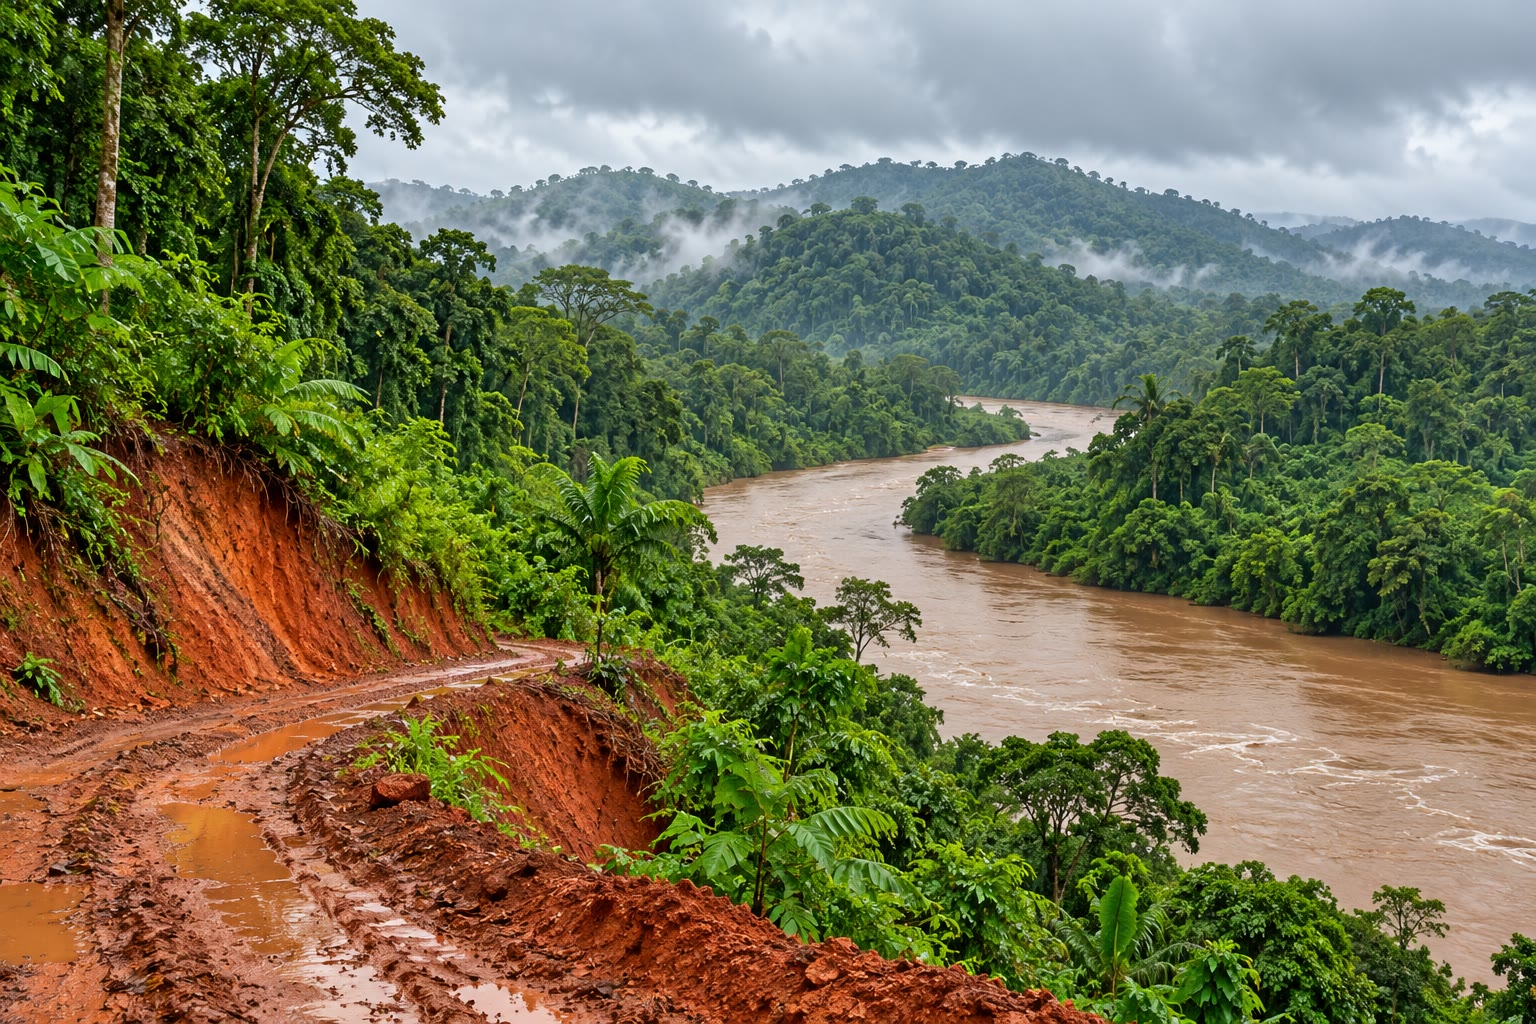
\includegraphics[width=0.66\linewidth]{images/book4/ai/b2-tropical-weathering.jpg}
\par\smallskip{\small Donde el termostato trabaja con más intensidad: una llanura cálida y húmeda, donde la lluvia cae sobre
un suelo rojo profundamente meteorizado y el río lleva al mar los productos de la meteorización
(ilustración generada por IA).}
\end{omfigure}

\section*{Ejercicios}\label{sec:b2:deep-time-climate:exercises}

Datos de los ejercicios, salvo aviso contrario: carbono preindustrial en la atmósfera
\qty{591}{PgC} (\qty{278}{ppm}); $\qty{1}{Tmol}$ de carbono $= \qty{0.012011}{PgC}$; meteorización de
silicatos $W_0 = \qty{0.138}{PgC.yr^{-1}}$; fracción de un exceso que queda en el aire después del océano y los
carbonatos $f = 0.08$; sensibilidad de la meteorización $k_T = \qty{0.09}{K^{-1}}$; sensibilidad climática $S =
\qty{3}{K}$; forzamiento de una duplicación del dióxido de carbono \qty{3.93}{W.m^{-2}}; $R =
\qty{8.314}{J.mol^{-1}.K^{-1}}$.
% ledger: ar6ch5:fig512, ipcc:erf-2xco2, derry24:fluxes, colbourn13:timescale, colbourn13:weathering, ipcc:ecs

\begin{exercise}[$\star$]\label{exo:b2:deep-time-climate:1}
Antes de la era industrial, el océano contenía \qty{900}{PgC} en su capa superficial, \num{37100} en sus
aguas intermedias y profundas, 700 como carbono orgánico disuelto y 3 en sus organismos vivos.
(a) ¿Cuánto carbono contenía el océano, y cuántas veces el de la atmósfera? (b) Conviértanse los
\qty{3.5e6}{Tmol} de los reservorios superficiales a petagramos de carbono. (c) ¿Qué parte de ellos está en el
aire?
\end{exercise}

\begin{exercise}[$\star$]\label{exo:b2:deep-time-climate:2}
Úsense los flujos de la figura del \omterm{def:b2:deep-time-climate:carbon-cycle}{ciclo del carbono a largo plazo}, con la desgasificación metamórfica tomada como
\qty{3}{Tmol.yr^{-1}}. (a) Súmense las entradas a los reservorios superficiales y las salidas.
(b) ¿Qué parte de las entradas aportan los volcanes, los rifts y el \omterm{def:b2:metamorphic-facies:metamorphism}{metamorfismo}? (c) Hállese el tiempo de residencia
del carbono en los reservorios superficiales, usando las salidas.
\end{exercise}

\begin{exercise}[$\star$]\label{exo:b2:deep-time-climate:3}
(a) Escríbase la meteorización de la forsterita, \ce{Mg2SiO4}, por el dióxido de carbono y el agua para dar iones magnesio
y bicarbonato y sílice disuelta, \ce{SiO2}, y ajústese. (b) El magnesio se deposita después
como carbonato. Escríbase la reacción neta. (c) ¿Qué masa de forsterita hay que meteorizar para
retirar \qty{1}{PgC} de forma definitiva? ($M(\ce{Mg2SiO4}) = \qty{140.7}{g.mol^{-1}}$.)
\end{exercise}

\begin{exercise}[$\star$]\label{exo:b2:deep-time-climate:4}
Ordénense por edad, con sus fechas, e indíquese para cada uno si la Tierra estaba en un estado de invernadero o en un
estado glaciar: el Óptimo Climático del Eoceno Temprano; la glaciación hirnantiense; el inicio del casquete de hielo
antártico; el Turoniense; la máxima extensión del hielo del Paleozoico superior; los grandes
avances de los casquetes de hielo del norte; el PETM.
\end{exercise}

\begin{exercise}[$\star\star$]\label{exo:b2:deep-time-climate:5}
(a) Compruébese que una energía de activación de \qty{63}{kJ.mol^{-1}} a \qty{288}{K} da $k_T =
\qty{0.09}{K^{-1}}$. (b) Hállese $k_T$ para el valor de campo \qty{74}{kJ.mol^{-1}}. (c) Con cada uno, hállese
el calentamiento estacionario cuando la desgasificación aumenta un \qty{20}{\percent}. (d) ¿Por qué la sensibilidad
climática no interviene en (c)?
\end{exercise}

\begin{exercise}[$\star\star$]\label{exo:b2:deep-time-climate:6}
Compárese el factor de Arrhenius exacto $\exp[-(E_{\text a}/R)(1/T - 1/T_0)]$ con $e^{k_T(T -
T_0)}$, $k_T = E_{\text a}/(RT_0^2)$, para $E_{\text a} = \qty{63}{kJ.mol^{-1}}$ y $T_0 =
\qty{288}{K}$: (a) en $T = \qty{293}{K}$; (b) en $T = \qty{318}{K}$. (c) Demuéstrese que la razón entre la
aproximación y el factor exacto es $\exp[E_{\text a}x^2/(RT_0^2(T_0 + x))]$, con $x = T - T_0$,
y hállese el calentamiento para el que alcanza 1.1.
\end{exercise}

\begin{exercise}[$\star\star$]\label{exo:b2:deep-time-climate:7}
La compilación suavizada da \qty{1444}{ppm} de dióxido de carbono a \qty{419.5}{Ma} y
\qty{276}{ppm} al final de su registro. (a) Hállese el forzamiento de ese descenso. (b) Compárese con
los \qty{9}{W.m^{-2}} del Sol que gana brillo. (c) Hállese el ritmo medio de descenso en ppm por millón de
años, y compárese con los \qty{3.4}{ppm} de la tendencia ajustada. ¿Por qué pueden diferir?
\end{exercise}
% ledger: data:b4-foster2017, foster17:co2

\begin{exercise}[$\star\star$]\label{exo:b2:deep-time-climate:8}
(a) Repártanse \num{3000} y \qty{7000}{PgC} a lo largo de 3 y de \qty{20}{kyr}: ¿qué intervalo de ritmos de
emisión resulta? Compárese con el intervalo de 0.3 a \qty{1.5}{PgC.yr^{-1}} que cita el IPCC. (b) Las emisiones humanas
fueron de unas \qty{35}{Gt} de dióxido de carbono en 2010. Conviértanse a carbono y compárense. (c) El dióxido de
carbono subió de 900 a \qty{2000}{ppm}. Hállense el forzamiento y el calentamiento de equilibrio con $S =
\qty{3}{K}$, y compárense con los \qty{5}{\celsius} de calentamiento sobre el clima anterior al PETM.
\end{exercise}
% ledger: ar6ch5:petm-release, usgs:volcanic-co2, ar6ch5:petm

\begin{exercise}[$\star\star$]\label{exo:b2:deep-time-climate:9}
El levantamiento de una cordillera multiplica por 1.2 la meteorizabilidad $W_0$ de la Tierra, con una
desgasificación constante. (a) Hállese el nuevo cambio de temperatura estacionario. (b) Hállese el nuevo dióxido de carbono estacionario, a partir de
\qty{278}{ppm}. (c) ¿Difiere la velocidad de la meteorización de silicatos, en el nuevo estado estacionario, de la
antigua? Explíquese.
\end{exercise}

\begin{exercise}[$\star\star\star$]\label{exo:b2:deep-time-climate:10}
(a) Hállese el tiempo característico del termostato con el factor de escorrentía, $k = 0.09 + 0.65\times0.045$.
(b) A lo largo de millones de años, los casquetes de hielo y la vegetación también responden; con una sensibilidad del
sistema Tierra de \qty{8}{K} por duplicación en lugar de $S$, hállese $\tau$ con $k_T$. (c) ¿En qué sentido empujan
al termostato los dos cambios, y qué incertidumbre, la de $E_{\text a}$ o la de $S$, pesa más?
\end{exercise}

\begin{exercise}[$\star\star\star$]\label{exo:b2:deep-time-climate:11}
Una emisión de \qty{5000}{PgC} (después del océano y los carbonatos). (a) Hállense el dióxido de carbono del
aire, en ppm, y el calentamiento. (b) Hállese la velocidad neta inicial de retirada $W - W_0$, y el tiempo que el
pulso tardaría en desaparecer a ese ritmo. (c) Hállese el tiempo linealizado para retirar el \qty{90}{\percent}
del exceso. (d) El modelo, integrado sin linealizar, tarda \qty{340}{kyr}. ¿Por qué más?
\end{exercise}

\begin{exercise}[$\star\star\star$]\label{exo:b2:deep-time-climate:12}
(a) Linealícese el modelo en torno a un estado estacionario en el que la desgasificación es $V$ y $C = C^*$, y demuéstrese que
el tiempo característico es $\tau' = A_0 (C^*/C_0)\ln 2/(f k S V)$. (b) Evalúese para el estado estacionario
de una subida de la desgasificación del \qty{20}{\percent}. (c) ¿Es el termostato más rápido o más lento en un mundo rico en
dióxido de carbono, y por qué?
\end{exercise}

\begin{problem}[{Problema de fin de semana --- ¿Cuánto tarda el termostato?}]\label{pb:b2:deep-time-climate:1}
Este problema construye la constante de tiempo del termostato a partir de flujos medidos. Úsense los datos de los
ejercicios; desgasificación en dorsales, \omterm{def:b2:oceanic-islands:stages}{islas oceánicas}, arcos y rifts: \num{1.3}, \num{1.3}, 4.5 y
\qty{4.2}{Tmol.yr^{-1}}; meteorización de silicatos, de 11 a \qty{12}{Tmol.yr^{-1}}; energía de activación,
\qty{63}{kJ.mol^{-1}} a $T_0 = \qty{288}{K}$; masa de la atmósfera, \qty{5.1e18}{kg}; masa molar media
del aire, \qty{28.97}{g.mol^{-1}}. Redondéese a tres cifras significativas.

\noindent\textbf{Parte I --- Balance.}
\begin{enumerate}
  \item Súmese la desgasificación volcánica y de los rifts, en \unit{Tmol.yr^{-1}} y en \unit{PgC.yr^{-1}}.
  \item Tómese $W_0$ en el centro de su intervalo; conviértase a \unit{PgC.yr^{-1}}.
  \item Compárense ambas. ¿Qué sugiere la comparación sobre el \omterm{def:b2:deep-time-climate:carbon-cycle}{ciclo del carbono a largo plazo}?
  \item ¿Cuántos moles de aire contiene la atmósfera? ¿Cuántos moles de carbono son \qty{591}{PgC},
        y a qué \omterm{def:b2:atmospheric-thermodynamics:moist-air}{razón de mezcla} corresponde?
  \item Sin ninguna meteorización, ¿cuánto tardaría la desgasificación de la pregunta 1 en añadir
        \qty{591}{PgC} a los reservorios superficiales?
  \item Si una fracción $f = 0.08$ de ese carbono permaneciera en el aire, ¿en qué factor aumentaría el dióxido de carbono
        del aire?
\end{enumerate}

\noindent\textbf{Parte II --- La linealización.}
\begin{enumerate}[resume]
  \item Hállese $k_T$ a partir de la energía de activación, y compruébese que redondeado da los
        \qty{0.09}{K^{-1}} usados más abajo.
  \item ¿En qué factor crece la meteorización para un calentamiento de \qty{1}{K}?
  \item Escríbase el calentamiento $\Delta T$ para un exceso $M$, y su derivada en $M = 0$, en
        \unit{K.PgC^{-1}}.
  \item Hállese la derivada de $W$ respecto de $M$ en $M = 0$, en \unit{yr^{-1}}.
  \item Demuéstrese que su inversa es la constante de tiempo $\tau$ de la
        \cref{prop:b2:deep-time-climate:thermostat}.
  \item ¿Cuáles de $f$, $k$, $S$ y $W_0$ hacen más rápido el termostato cuando aumentan?
\end{enumerate}

\noindent\textbf{Parte III --- La constante de tiempo.}
\begin{enumerate}[resume]
  \item Evalúese $\tau$.
  \item Evalúese con el factor de escorrentía, $k = \qty{0.119}{K^{-1}}$.
  \item Evalúese con $k_T$ y una energía de activación de \qty{74}{kJ.mol^{-1}}.
  \item Compárense estos valores con el intervalo de \qty{200}{kyr} a \qty{1}{Myr} de los modelos con un océano explícito.
  \item ¿Cuántos tiempos característicos caben en los \qty{50}{Myr} del descenso cenozoico del dióxido
        de carbono? ¿Qué dice eso del estado del ciclo del carbono durante el descenso?
  \item A \qty{16}{ppm} por millón de años, ¿cuánto cambia el dióxido de carbono en un $\tau$?
\end{enumerate}

\noindent\textbf{Parte IV --- Una emisión del tamaño del PETM.}
\begin{enumerate}[resume]
  \item Se emiten \qty{5000}{PgC}; ¿cuánto queda en el aire después de que hayan actuado el océano y los carbonatos,
        y cuál es el dióxido de carbono en ppm?
  \item Hállese el calentamiento en ese momento.
  \item ¿Cuánto aumenta la velocidad de meteorización, en \unit{PgC.yr^{-1}} y en porcentaje?
  \item Con la ley linealizada, ¿cuánto tiempo pasa hasta que desaparece el \qty{90}{\percent} del exceso?
  \item Los carbonatos del PETM se recuperaron a lo largo de unos \qty{100}{kyr}. Dense dos razones por las que la Tierra
        real pudo ser más rápida que este modelo.
  \item En resumen: ¿cuál es el tiempo característico del \omterm{def:b2:deep-time-climate:thermostat}{termostato de la meteorización de los silicatos} en este modelo?
\end{enumerate}
\end{problem}
% ledger: derry24:fluxes, colbourn13:weathering, colbourn13:timescale, ar6ch5:fig512, ar6ch5:petm, ar6ch5:cenozoic-co2, ipcc:ecs, earth:Matm, earth:Mmol
